\documentclass[lettersize,journal]{IEEEtran}
\usepackage{amsmath,amsfonts}
\usepackage{algorithmic}
\usepackage{algorithm}
\usepackage{array}
\usepackage[caption=false,font=normalsize,labelfont=sf,textfont=sf]{subfig}
\usepackage{textcomp}
\usepackage{stfloats}
\usepackage{url}
\usepackage{verbatim}
\usepackage{graphicx}
\usepackage{cite}
\usepackage{booktabs}
\usepackage{tikz}
\usetikzlibrary{positioning,arrows.meta}
\hyphenation{op-tical net-works semi-conduc-tor IEEE-Xplore}

\begin{document}

\title{Reproducing and Extending the Clue of Emotion (CoE) Framework for Emotion Recognition in Conversations on a Single Consumer GPU}

\author{Kishor Koppikar, [Roll No.]% <-- add roll number / co-authors
\thanks{Project report. Contact: kishorkoppikar@gmail.com}}

\maketitle

\begin{abstract}
Emotion Recognition in Conversations (ERC) with large language models benefits from textual clues such as speaker personas and scene descriptions, and from multi-stage auxiliary training. We implement the Clue of Emotion (CoE) framework with its mixed auxiliary strategy (self-taught rationale generation, joint auxiliary training, then a separate ERC stage) for EmoryNLP, MELD and IEMOCAP on a single 12\,GB GPU using 4-bit QLoRA on Mistral-7B. Our pipeline reaches weighted F1 of 40.00 (EmoryNLP), 67.35 (MELD) and 69.97 (IEMOCAP) against reported 44.29, 70.11 and 70.46. We then test three extensions under a controlled protocol with shuffled-clue controls and paired-bootstrap intervals: chain-of-emotion targets, character-relationship clues and acoustic clues. None improves the base at full training length. Chain of emotion does improve accuracy significantly in a short, low-data protocol ($+2.4$ to $+4.5$ weighted F1 on EmoryNLP and IEMOCAP), but the advantage disappears with full training. Changing training length, LoRA rank or the base model did not close the remaining EmoryNLP gap.
\end{abstract}

\begin{IEEEkeywords}
Emotion recognition in conversation, large language models, QLoRA, chain of emotion, reproducibility.
\end{IEEEkeywords}

%% ------------------------------------------------------------------
\section{Introduction}
Emotion Recognition in Conversations (ERC) assigns an emotion label to each utterance of a dialogue and underlies applications such as virtual assistants and mental-health monitoring. Large language models (LLMs) fine-tuned for ERC are strong, but they are limited by how well they interpret long conversational streams. The CoE framework~\cite{coe2025} addresses this by adding global textual clues (speaker persona and scene) to the prompt and by training in several stages with auxiliary tasks: speaker identification, role-play, and self-taught emotion reasoning.

This project asks two questions. First, can the CoE pipeline be reproduced on commodity hardware (one RTX 3060, 12\,GB, 16\,GB RAM) rather than the 8$\times$32\,GB V100 cluster of the original work, and how close does it get? Second, can simple additional clues or targets improve it? We implement the full pipeline for three benchmarks, build three extensions, and evaluate each with controls and confidence intervals so that small differences are not over-interpreted.

\textbf{Contributions.}
(i) A complete, resumable implementation of the CoE mixed auxiliary strategy for EmoryNLP, MELD and IEMOCAP that runs on 12\,GB, including locally generated scenes and seed rationales and an IEMOCAP scene clue aligned to turns.
(ii) A controlled study of three extensions with shuffled-clue controls and paired-bootstrap intervals.
(iii) Negative results on closing the EmoryNLP gap (more epochs, higher rank, a different base model), reported with their uncertainty.

%% ------------------------------------------------------------------
\section{Related Work}
\textbf{ERC models.} Early ERC systems used hand-crafted features and recurrent or graph models that track speaker state and interactions, such as DialogueRNN~\cite{dialoguernn2019}, DialogueGCN~\cite{dialoguegcn2019} and COSMIC~\cite{cosmic2020}. More recently LLMs have been fine-tuned or prompted for ERC; InstructERC~\cite{instructerc2023} reformulates ERC as instruction following with retrieval and multi-task training.

\textbf{Clues and auxiliary tasks.} CoE~\cite{coe2025} adds persona and scene clues, and trains with role-play, speaker identification and rationale tasks in multi-stage strategies. The rationale task follows the self-taught reasoner idea~\cite{star2022}, in which a model generates its own rationales and keeps those that lead to correct answers; chain-style reasoning in general is motivated by chain-of-thought prompting~\cite{cot2022}.

\textbf{Efficient fine-tuning.} Low-rank adapters~\cite{lora2022} and 4-bit quantised base weights~\cite{qlora2023}, together with optimiser sharding~\cite{zero2020}, make 7B-parameter models trainable on a single consumer GPU. We use these to run CoE on 12\,GB, at the cost of the precision and compute budget of the original setup (Section~\ref{sec:setup}).

%% ------------------------------------------------------------------
\section{Proposed Methodology}
\subsection{Base pipeline: CoE mixed auxiliary strategy}
All variants share the same pipeline (Fig.~\ref{fig:pipeline}). \emph{Prompt format}: the ERC prompt contains the instruction, speaker personas and a scene description (clues), the dialogue history, the current utterance, and the label set; the target is the emotion label (Appendix~A).
\begin{enumerate}
\item \textbf{Scene and seed data.} Scenes for EmoryNLP and MELD are generated by a local Mistral model from the first three utterances only (physical setting only, with a filter banning emotion words). IEMOCAP has no persona; its scene clue is recovered from the session scripts and aligned to turns. Seed rationales are generated locally.
\item \textbf{STEeR loop.} A self-taught loop trains on seed rationales, then repeatedly infers rationales for unseen training utterances and keeps those whose predicted label is correct.
\item \textbf{Stage 1 (auxiliary).} Joint training on speaker identification, role-play (generate the next line in a given emotion) and the collected rationales.
\item \textbf{Stage 2 (ERC).} Starting from the stage-1 adapter, train on the ERC task alone and evaluate each epoch.
\end{enumerate}

\begin{figure}[!t]
\centering
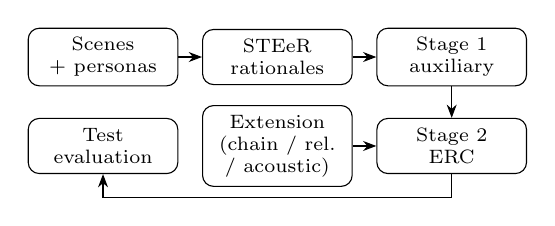
\begin{tikzpicture}[node distance=3mm, box/.style={draw, rounded corners, font=\scriptsize, align=center, minimum width=1.9cm, minimum height=0.7cm}, >=Stealth]
\node[box] (a) {Scenes\\+ personas};
\node[box, right=of a] (b) {STEeR\\rationales};
\node[box, right=of b] (c) {Stage 1\\auxiliary};
\node[box, below=4mm of c] (d) {Stage 2\\ERC};
\node[box, left=of d] (e) {Extension\\(chain / rel.\\/ acoustic)};
\node[box, left=of e] (f) {Test\\evaluation};
\draw[->] (a)--(b); \draw[->] (b)--(c); \draw[->] (c)--(d);
\draw[->] (e)--(d); \draw[->] (d.south) -- ++(0,-3mm) -| (f.south);
\end{tikzpicture}
\caption{Pipeline. Extensions change only the stage-2 prompt or target; stage 1 is reused.}
\label{fig:pipeline}
\end{figure}

\subsection{Extensions}
Every extension reuses the same stage-1 adapter and hyper-parameters, so a run differs from the base \emph{only} in the stage-2 prompt or target.
\begin{itemize}
\item \textbf{Chain of emotion.} The target first lists emotions of earlier turns and then the current emotion (final label read from the line ``Current Emotion:''). Variants: \emph{self} (the current speaker's earlier turns), \emph{prev} (the preceding turn only), \emph{all} (every earlier turn), \emph{all-known} (like \emph{all} but skipping IEMOCAP turns without a gold emotion), and \emph{label-first} versions (\emph{lf-all}, \emph{lf-prev}) that emit the current label first and the chain afterwards.
\item \textbf{Character relationships.} A short block describing relationships among the main characters (curated maps in detail, category and description styles) is added to the prompt.
\item \textbf{Acoustic clues.} Per-utterance audio features (pitch, loudness, speaking rate, and their variation) are turned into short text, either a compact factual \emph{description} or an interpretive \emph{impression}; optional tags can be added to the last three context turns. Thresholds are percentile based, globally or per speaker.
\end{itemize}
For each clue extension a \emph{shuffled control} places the same clue text on random turns, so that any gain must come from the clue content and not from added tokens.

%% ------------------------------------------------------------------
\section{Experimental Setup}\label{sec:setup}
\textbf{Datasets.} EmoryNLP~\cite{emorynlp2018} (7 emotions; 9{,}934 / 1{,}344 / 1{,}328 utterances in train/dev/test), MELD~\cite{meld2019} (7 emotions; 9{,}989 / 1{,}109 / 2{,}610) and IEMOCAP~\cite{iemocap2008} (6 emotions; 5{,}758 / 1{,}622 / 1{,}622). We use the standard splits; in the IEMOCAP split we use, the dev and test files have the same size (1{,}622 utterances). The metric is weighted F1.

\textbf{Model and training.} Mistral-7B-Instruct-v0.3 in 4-bit NF4 with LoRA (rank 8, $\alpha=16$), learning rate $2\times10^{-4}$, DeepSpeed ZeRO-2, batch 2 with 8 accumulation steps, maximum length 1400. Stage 1 uses 2 epochs on 50\,\% of the auxiliary data; stage 2 uses 3 epochs on all data. The full EmoryNLP pipeline takes about 23\,GPU-hours on the RTX 3060; a single stage-2 arm takes about 12 hours (EmoryNLP/MELD) or 4--5 hours (IEMOCAP).

\textbf{Deviations from the reference setup.} The reference setup uses fp16, LoRA rank 16, 20 ERC epochs, frontier-model scenes and rationales, and averages three independent runs~\cite{coe2025}. We use 4-bit weights, 3 epochs, locally generated scenes and rationales and a \emph{single} run per arm. Absolute scores are therefore not directly comparable.

\textbf{Statistics.} Arms are compared by the \emph{final} epoch (to avoid test-set epoch selection) using a paired bootstrap over test rows (1000 resamples, 95\,\% interval). Because there is one run per arm, intervals capture test-sampling noise only; differences below about 1--2 points should be treated as noise.

\textbf{Short protocol.} For ablations we use 1 epoch on 30\,\% of the training data, scored on held-out dev rows (EmoryNLP and MELD dev sets; IEMOCAP: every fifth training dialogue). Every arm starts from the same stage-1 adapter. The reference arm \emph{nocue} is the same fine-tune with no added clue or chain.

%% ------------------------------------------------------------------
\section{Results and Analysis}
\subsection{Base pipeline}
Table~\ref{tab:base} compares our base pipeline with the reported scores. IEMOCAP and MELD come within 0.5 and 2.8 points; EmoryNLP is 4.3 points lower.

\begin{table}[!t]
\caption{Base pipeline, test weighted F1 (final epoch).}\label{tab:base}
\centering\small
\begin{tabular}{lccc}
\toprule
Dataset & Ours & Best epoch & Reported~\cite{coe2025}\\
\midrule
EmoryNLP & 40.00 & 40.00 & 44.29\\
MELD & 67.35 & 67.76 & 70.11\\
IEMOCAP & 69.97 & 69.97 & 70.46\\
\bottomrule
\end{tabular}
\end{table}

\subsection{Attempts to close the EmoryNLP gap}
We tested the three most likely explanations for the EmoryNLP gap (Table~\ref{tab:gap}). None moves the score beyond noise.

\begin{table}[!t]
\caption{EmoryNLP: attempts to close the gap (test, final epoch). $\Delta$ is relative to the base with its 95\,\% interval.}\label{tab:gap}
\centering\small
\begin{tabular}{lcl}
\toprule
Change & wF1 & $\Delta$ [95\,\% CI]\\
\midrule
Base (v0.3, r=8, 3 ep.) & 40.00 & --\\
Continued to 8 epochs & 39.27 & $-0.81$ [$-2.71$, $+1.06$]\\
LoRA rank 16 (retrained) & 38.55 & $-1.42$ [$-3.67$, $+0.60$]\\
Mistral-7B-v0.1, 3 ep. & 39.79 & $-0.21$ [$-2.31$, $+2.13$]\\
Mistral-7B-v0.1, 6 ep. & 40.16 & $+0.18$ [$-2.26$, $+2.69$]\\
\bottomrule
\end{tabular}
\end{table}

When training is resumed, the optimiser and learning-rate schedule restart (a warm restart), which produces a temporary drop at the first resumed epoch: the v0.1 run goes 39.79 $\to$ 37.82 $\to$ 38.96 $\to$ 40.16 over epochs 2--5. Remaining differences from the reference setup (4-bit versus fp16 and 3 versus 20 ERC epochs) could not be tested in the available time.

\subsection{Extensions at full length}
Table~\ref{tab:chain} gives final-epoch differences to the base for chain of emotion. No chain variant is significantly better than the base on any dataset. \emph{All} and \emph{label-first all} are significantly worse on EmoryNLP and IEMOCAP, and \emph{self} on MELD.

\begin{table*}[!t]
\caption{Chain of emotion at full length (3 epochs): final-epoch $\Delta$ wF1 vs.\ base [95\,\% CI]. $^{*}$ = interval excludes 0.}\label{tab:chain}
\centering\small
\begin{tabular}{lccc}
\toprule
Variant & EmoryNLP & MELD & IEMOCAP\\
\midrule
chain-all & $-3.53$ [$-6.10$, $-0.95$]$^{*}$ & $-1.15$ [$-2.54$, $+0.36$] & $-3.81$ [$-5.88$, $-1.70$]$^{*}$\\
chain-prev & $-1.69$ [$-3.97$, $+0.61$] & $-0.78$ [$-2.24$, $+0.65$] & $-0.88$ [$-2.64$, $+0.92$]\\
chain-self & $-1.85$ [$-4.28$, $+0.50$] & $-1.98$ [$-3.37$, $-0.56$]$^{*}$ & $-1.27$ [$-3.04$, $+0.51$]\\
lf-all (label first) & $-3.44$ [$-6.03$, $-0.86$]$^{*}$ & -- & $-3.95$ [$-5.92$, $-2.00$]$^{*}$\\
\bottomrule
\end{tabular}
\end{table*}

Figure~\ref{fig:epochs} shows why: several chain arms start at or above the base after the first epoch (for example IEMOCAP chain-prev and lf-all, EmoryNLP chain-prev), but the base keeps improving while the chain arms flatten or fall.

\begin{figure*}[!t]
\centering
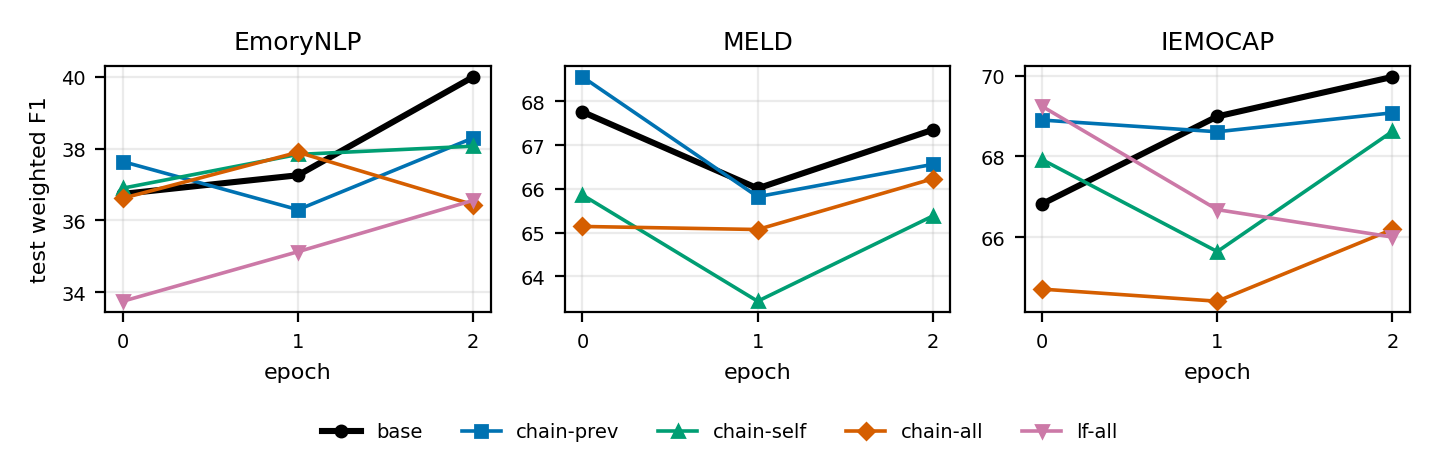
\includegraphics[width=0.85\textwidth]{fig_epochs}
\caption{Test weighted F1 per epoch at full length: the base (black) against the chain variants. The early advantage of chain targets does not persist.}
\label{fig:epochs}
\end{figure*}

On Mistral-7B v0.1 (EmoryNLP, 3 epochs, Table~\ref{tab:v01}), chain-all is again significantly worse ($-3.46$), and the relationship and acoustic arms are not distinguishable from the base. The acoustic arm has the highest EmoryNLP score of the study (41.42), but its interval includes zero ($+1.62$ [$-0.45$, $+3.79$]) and the controlled ablations below show no acoustic effect, so we regard it as unconfirmed.

\begin{table}[!t]
\caption{EmoryNLP with Mistral-7B v0.1, test wF1 per epoch; $\Delta$ vs.\ v0.1 base at epoch 2.}\label{tab:v01}
\centering\small
\begin{tabular}{lcccl}
\toprule
Arm & Ep.0 & Ep.1 & Ep.2 & $\Delta$ [95\,\% CI]\\
\midrule
Base & 36.08 & 38.88 & 39.79 & --\\
Acoustic & 36.67 & 39.65 & 41.42 & $+1.62$ [$-0.45$, $+3.79$]\\
Relation map & 36.85 & 39.58 & 39.43 & $-0.34$ [$-2.32$, $+1.66$]\\
Chain-prev & 37.03 & 38.45 & 38.26 & $-1.44$ [$-3.82$, $+0.95$]\\
Chain-all & 34.16 & 34.70 & 36.27 & $-3.46$ [$-5.88$, $-1.01$]$^{*}$\\
\bottomrule
\end{tabular}
\end{table}

%% ------------------------------------------------------------------
\section{Ablation Study}
The short protocol (Section~\ref{sec:setup}) tests each design choice against the no-clue fine-tune and, for clue arms, against its shuffled control. Table~\ref{tab:abl} summarises representative arms.

\begin{table}[!t]
\caption{Short-protocol ablation, dev wF1 and $\Delta$ vs.\ \emph{nocue} [95\,\% CI]. $^{*}$ = interval excludes 0.}\label{tab:abl}
\centering\footnotesize
\begin{tabular}{llcl}
\toprule
Data & Arm & wF1 & $\Delta$ vs.\ nocue\\
\midrule
EmoryNLP & nocue & 39.44 & --\\
 & lf-all & 41.95 & $+2.57$ [$+0.81$, $+4.48$]$^{*}$\\
 & chain-all & 41.85 & $+2.44$ [$+0.45$, $+4.45$]$^{*}$\\
 & lf-prev & 41.11 & $+1.69$ [$+0.04$, $+3.24$]$^{*}$\\
 & chain-prev & 40.19 & $+0.73$ [$-0.95$, $+2.52$]\\
 & relation map & 39.73 & $+0.30$ [$-0.89$, $+1.52$]\\
 & acoustic desc. & 39.34 & $-0.07$ [$-1.24$, $+1.09$]\\
 & acoustic, shuffled & 38.68 & $-0.75$ [$-2.00$, $+0.35$]\\
\midrule
IEMOCAP & nocue & 60.24 & --\\
 & chain-all & 64.67 & $+4.46$ [$+2.23$, $+6.75$]$^{*}$\\
 & chain-all-known & 64.26 & $+4.00$ [$+1.63$, $+6.51$]$^{*}$\\
 & lf-all & 64.11 & $+3.94$ [$+1.74$, $+6.07$]$^{*}$\\
 & lf-prev & 62.09 & $+1.83$ [$-0.01$, $+3.66$]\\
 & chain-prev & 58.54 & $-1.66$ [$-3.85$, $+0.61$]\\
 & acoustic desc. & 59.31 & $-0.95$ [$-2.68$, $+0.84$]\\
\midrule
MELD & nocue & 68.97 & --\\
 & lf-all & 69.20 & $+0.26$ [$-1.64$, $+2.15$]\\
 & chain-prev & 65.81 & $-3.19$ [$-5.34$, $-1.03$]$^{*}$\\
 & other arms & -- & no significant gain\\
\bottomrule
\end{tabular}
\end{table}

\textbf{Chain of emotion.} Chain targets help significantly in the short protocol on EmoryNLP and IEMOCAP ($+2.4$ to $+4.5$) but not on MELD, and the gain is gone after three epochs on full data (Table~\ref{tab:chain}). A plausible reading is that the extra supervision speeds up early learning, after which the base catches up.

\textbf{Acoustic clues.} We ablated the clue form (description, impression, both), the audio tags on context turns, removing the pitch, volume or speech-rate features, 3 versus 5 percentile classes and global versus per-speaker thresholds, each against no clue and a shuffled control, on all three datasets. No variant is reliably better than no clue or than its shuffled control; several are worse (e.g.\ on IEMOCAP the default impression form is $-2.60$ [$-4.78$, $-0.57$] and the shuffled description form is $-3.93$ [$-5.67$, $-2.23$]). We therefore did not run acoustic clues at full length on the Mistral-7B-Instruct-v0.3 base; the single full-length v0.1 run above is inconclusive.

\textbf{Relationship clues.} The relation map is indistinguishable from its shuffled control (relmap $+0.30$ vs.\ shuffled relmap $-0.19$ on EmoryNLP); the more verbose description style is significantly worse ($-1.86$ [$-3.22$, $-0.52$]).

%% ------------------------------------------------------------------
\section{Discussion}
\textbf{Reproduction.} On 12\,GB, 4-bit QLoRA, a smaller compute budget and locally generated auxiliary data, the pipeline gets within about 0.5 points on IEMOCAP and 2.8 on MELD of the reported scores. The remaining EmoryNLP gap (4.3 points) was not explained by more epochs, a higher rank or the v0.1 base model; each change was within noise. The most likely causes are precision (4-bit versus fp16), the number of ERC epochs (3 versus 20), differences in the generated scenes and rationales, and the fact that reported scores are averaged over three runs.

\textbf{Why extensions did not help.} Added clues did not beat their shuffled controls, which suggests the model does not extract useful information from them under this setup. Chain targets give a real early-training benefit but also lengthen the target and the evaluation generation, and at full length they trade away accuracy on the final label. Practically, chain of emotion may be useful when compute or data is limited; it is not a way to raise the converged score here.

\textbf{Evaluation practice.} Comparing best epochs chosen on the test set overstated several effects (for example a seemingly significant ensemble gain became $+0.19$, not significant, when final epochs were used). We therefore report final-epoch comparisons with paired-bootstrap intervals throughout.

%% ------------------------------------------------------------------
\section{Limitations}
\begin{itemize}
\item One training run per arm and no seed variance; reported intervals reflect test sampling only, and differences under about 1--2 points are noise.
\item Scene descriptions and seed rationales come from a local 7B model and are weaker than frontier-model outputs; EmoryNLP and MELD share the same synthetic-scene approach.
\item Short-protocol numbers are on dev rows with 30\,\% of the data and one epoch; they cannot be compared with test scores.
\item Resumed runs use a restarted learning-rate schedule and are not equal to a single long run.
\item Not tested: fp16 or 8-bit training, 20 ERC epochs, and multiple seeds. Extensions on v0.1 were run for EmoryNLP only.
\end{itemize}

%% ------------------------------------------------------------------
\section{Conclusion and Future Work}
A complete CoE Strategy~B pipeline can be implemented and run on a single 12\,GB GPU, reaching 40.00 / 67.35 / 69.97 weighted F1 on EmoryNLP / MELD / IEMOCAP. Three extensions (chain of emotion, relationship clues, acoustic clues) do not improve the converged score; chain of emotion improves early-training accuracy significantly on two datasets. Future work: multiple seeds for tighter conclusions; fp16 or 8-bit training with more ERC epochs to test the remaining EmoryNLP gap; frontier-model scenes and rationales; and full-length acoustic runs on additional datasets.

%% ------------------------------------------------------------------
\bibliographystyle{IEEEtran}
\bibliography{ref}

%% ------------------------------------------------------------------
\appendices
\section{Prompts and AI-Assistant Use}

\subsection*{A.1 Prompts used inside the pipeline}
The model prompts used for training are shown below (abbreviated where marked).

\noindent\textbf{ERC prompt (stage 2 and evaluation):}
\begin{small}\begin{verbatim}
As an expert in Conversational Emotion Recognition
(ERC), your task is to predict the emotion by analyzing
the Speaker Persona, Scene and Dialogue History
information.
### Speaker Persona: <persona per main character>
### Scene: <generated scene>
### Dialogue History: <previous turns>
### Current Utterance: <speaker: text>
Based on the context, what is the emotion of the current
utterance?
Choose from: <label set>
Answer with just the emotion label.
\end{verbatim}\end{small}

\noindent\textbf{Speaker identification (stage 1):}
\begin{small}\begin{verbatim}
You are now an expert in Conversational Emotion
Recognition. Your task is to predict the speaker by
analyzing sentences. Here's a list of individuals and
their Speaker Persona ...
Please select the Speaker of <"text", Emotion: label>
from <candidates>.
\end{verbatim}\end{small}

\noindent\textbf{Role-play (stage 1):}
\begin{small}\begin{verbatim}
You are now an expert role-play actor. Analyze the
character's Speaker Persona, Scene, and Dialogue History
to predict their most likely next line.
... You will stay in character whenever possible, and
generate responses in <emotion> emotion as if you were
<speaker>.
\end{verbatim}\end{small}

\noindent\textbf{Rationale (STEeR):}
\begin{small}\begin{verbatim}
Please analyze the emotional state of <speaker: "text">
by first providing your rationale based on the given
context, then select the emotional label from <labels>.
\end{verbatim}\end{small}

\noindent\textbf{Scene generation (local Mistral):}
\begin{small}\begin{verbatim}
Below are the opening lines of a scene from the TV
sitcom Friends. In ONE short sentence (max 20 words),
state only the physical setting where it takes place,
and who is present if clear. Do not mention emotions,
mood, plot or relationships. If the setting is neither
stated nor clearly implied, answer exactly:
Unknown setting
\end{verbatim}\end{small}

\subsection*{A.2 AI assistant and platforms}
\begin{itemize}
\item \textbf{Models:} Mistral-7B-Instruct-v0.3 (main experiments) and Mistral-7B-v0.1 (base-model check), run locally.
\item \textbf{Compute:} one RTX 3060 (12\,GB) and a second desktop for parallel arms.
\item \textbf{Software:} PyTorch, Transformers, PEFT, bitsandbytes, DeepSpeed (versions pinned in the repository).
\item \textbf{AI assistant:} Claude Code (Anthropic) was used as a coding and analysis assistant throughout the project: implementing and reviewing the pipeline and extensions, writing the evaluation and bootstrap scripts, checking results for errors, and drafting this report. All experiments were launched and run by the author, and the author reviewed the results.
\end{itemize}

\end{document}
